\documentclass[a4paper]{article}

\usepackage[T1]{fontenc}
\usepackage[margin=2.5cm]{geometry}
\usepackage{abstract}
\usepackage{graphicx}

\author{The Unicorn Hunters\\
(Christian Frantzen, Guilherme Barreiro Vieira,\\
Mortimer Sotom and Théo Verhelst )}
\title{Advanced Machine Learning Coursework: Kaggle Competition NYC Taxis}

\begin{document}
\maketitle


\begin{abstract}
This is the abstract
\end{abstract}

\section{Introduction}

\section{Data Analysis}
The first step of a machine learning project is to explore and analyse the data,
in order to better understand the problem. Our dataset is composed of 11
features: a unique identifier for each row, the identifier of the taxi company,
the pickup time, the pickup and drop-off locations, the number of passengers,
and a boolean flag indicated if the trip data has been stored on-board or
directly sent to the data server.

Figures XX to XX show the distribution of some of these features. We did not
show the pickup month, minute and seconds, as their graphs are uniformly
distributed and therefore not visually informative. Outliers have been removed
in order to properly display the pickup and drop-off location distribution, as
well as the trip duration. These outliers will be discussed in the next section.
We can see in figure \ref{long} and \ref{lat} that the location seems to be
roughly normally distributed, and the logarithm of the trip duration also
appears to be normally distributed in figure \ref{log_trip_duration}. The smaller
bumps outside of the main bell in the location curves correspond to trips to the
city airport.

\begin{figure}
    \centering
   \begin{minipage}{.45\textwidth}
        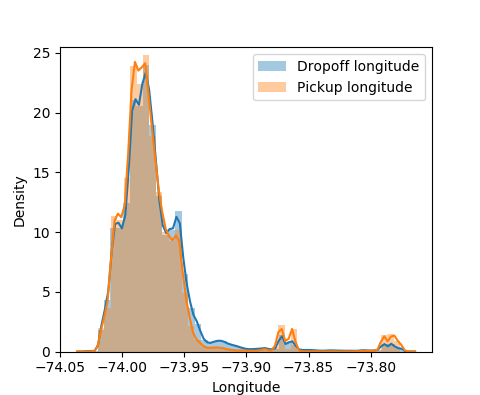
\includegraphics[width=\linewidth]{longitude}
        \caption{Distribtion of the longitude.}
        \label{long}
    \end{minipage}
    \hspace{0.05\textwidth}
    \begin{minipage}{.45\textwidth}
        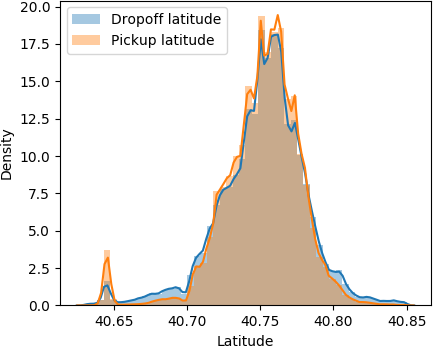
\includegraphics[width=\linewidth]{latitude}
        \caption{Distribution of the latitude.}
        \label{lat}
    \end{minipage}
\end{figure}

\begin{figure}
    \centering
    \begin{minipage}{.45\textwidth}
        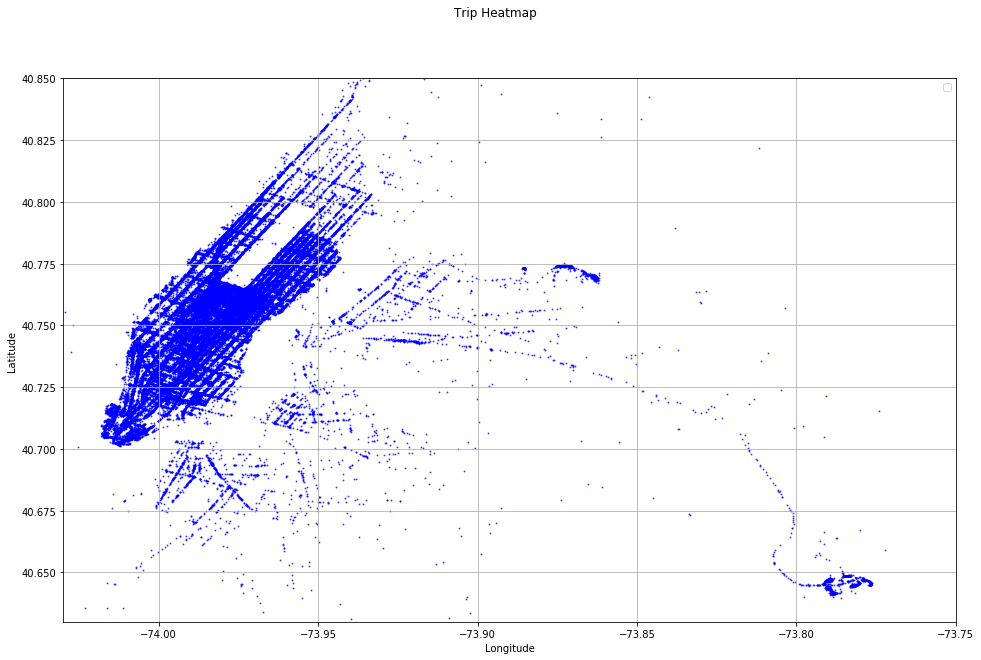
\includegraphics[width=\linewidth]{heatmap}
        \caption{Trip locations as distributed on a map.}
        \label{heatmap}
    \end{minipage}
    \hspace{0.05\textwidth}
   \begin{minipage}{.45\textwidth}
       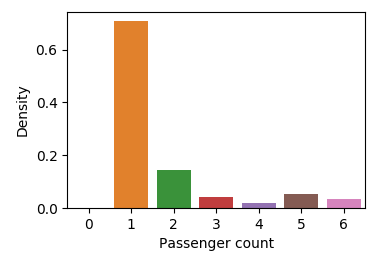
\includegraphics[width=\linewidth]{passenger_count}
       \caption{Distribution of the number of passengers.}
       \label{passenger_count}
    \end{minipage}
\end{figure}

\begin{figure}[h]
    \centering
    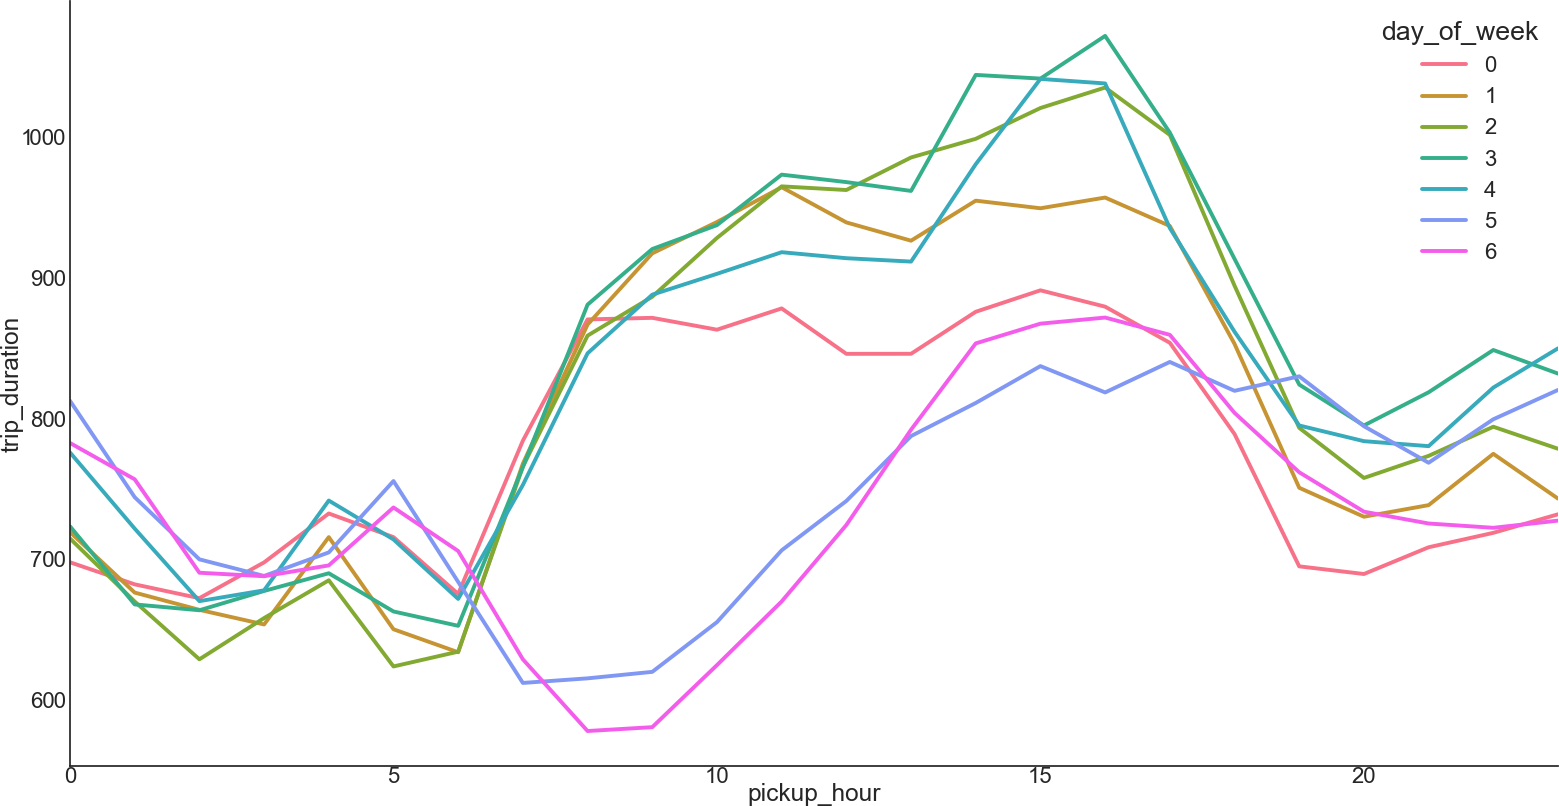
\includegraphics[width=\linewidth]{pickup_hour_vs_trip_duration}
    \caption{Distribution of the pickup time, for different days of the week.}
    \label{pickup_hour}
\end{figure}

\begin{figure}
    \centering
    \begin{minipage}{.45\textwidth}
        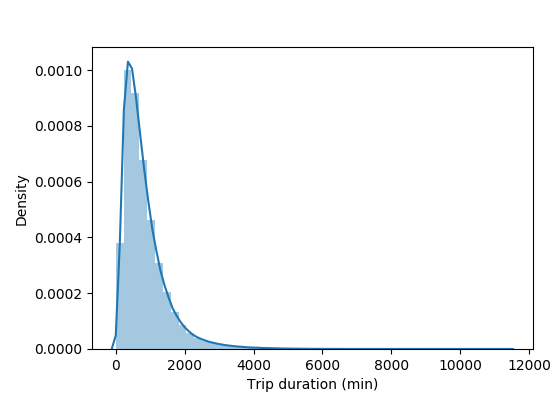
\includegraphics[width=\linewidth]{trip_duration}
        \caption{Distribution of the trip duration, in seconds.}
        \label{trip_duration}
    \end{minipage}
    \hspace{0.05\textwidth}
   \begin{minipage}{.45\textwidth}
       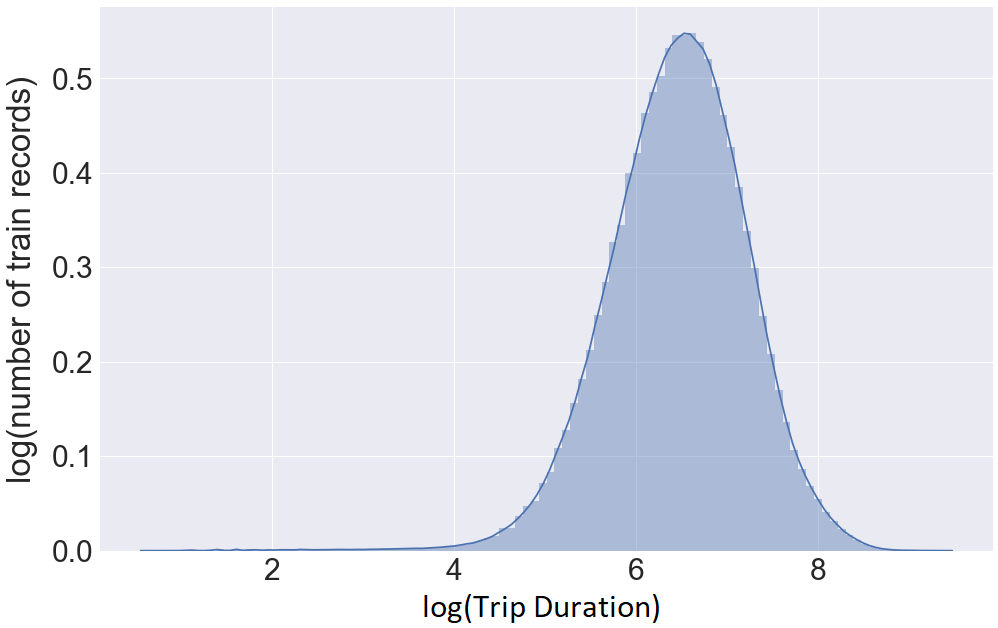
\includegraphics[width=\linewidth]{log_trip_duration}
       \caption{Distribution of the logarithm of the trip duration, in seconds.}
       \label{log_trip_duration}
    \end{minipage}
\end{figure}


It is also important to make sure that the training and test sets are
independently and identically distributed. For this, we compared the above
distributions with those from the test set. If the distribution from the
training and testing set significantly overlap, then we can consider that the
I.I.D. assumption is verified. As shown for example in figure
and , it is indeed the case.

\section{Preprocessing}

\section{Feature Selection}

\section{Methods for Model Selection}

\section{Results}

\section{Conclusion}

\newpage
\footnotesize
\bibliographystyle{ieeetr}
\bibliography{report}

\appendix
\newpage
\section{Additional Figures}

\end{document}
